\documentclass[12pt]{article}

\usepackage{scicite,times,graphicx,float,hyperref}
\usepackage[skip=0pt]{caption}
\usepackage[utf8]{inputenc}
\usepackage{enumitem}
\usepackage{booktabs}
\usepackage{multicol}

\topmargin -1.0cm
\oddsidemargin 0.0cm
\textwidth 16cm 
\textheight 23cm
\footskip 1.0cm

\newenvironment{sciabstract}{%
\begin{quote} \bf}
{\end{quote}}

\newcounter{lastnote}
\newenvironment{scilastnote}{%
  \setcounter{lastnote}{\value{enumiv}}%
  \addtocounter{lastnote}{+1}%
  \begin{list}%
  {\arabic{lastnote}.}
  {\setlength{\leftmargin}{.22in}}
  {\setlength{\labelsep}{.5em}}
}
{\end{list}}

\title{Simulation of a Scientific Computation Platform\\With a Focus on Quality Attributes} 

\author
{Filipe Pires [85122], João Alegria [85048]\\
\\
Software Architecture\\
\normalsize{Department of Electronics, Telecommunications and Informatics}\\
\normalsize{University of Aveiro}\\
} 

\date{\today{}}

%%%%%%%%%%%%%%%%% END OF PREAMBLE %%%%%%%%%%%%%%%%

\begin{document}

\baselineskip18pt

\maketitle

\section*{Introduction} %%%%%%%%%%%%%%%%%%%%%%%%%%%%%%%%%%%%%%%%%%%%%%%%%%%%%%%%%%%%%%%%%%%%%%%%%%%%%%%%%%%%%%%%%%%%%%%%%%%%%%%%%%%%%%%%%%%%%%%%%%%%%%%%%%%%%%%%

This report aims to describe the work developed for the second assignment of the course of 'Software Architecture', focused on a platform that collects and
processes information from simulated vehicles.

The aim of the assignment was to explore the capabilities of a technology like Kafka in standard IoT solutions.
The platform itself isn't meant to provide a field-tested solution to a problem or a set of problems, rather it is supposed to show how communications via Kafka
can empower developers in a time that modularity is more important than ever and system components must be prepared to easily transfer data streams between each other.

So in this report we present the architecture of our solution and the Kafka-related configurations, justifying them according to what we learned and found to be
most suitable for each specific use case.
We also mention how the work was distributed amongst the authors.

All code developed is publicly accessible in our GitHub repository:

\url{https://github.com/FilipePires98/AS/}

% \vspace{-10pt}
% \begin{itemize}[noitemsep]
%   \item Prepare - the selected farmers move to a Standing Area, ready for orders.
%   \item Start - the actual simulation begins and farmers start moving.
%   \item Collect - farmers collect corn cobs from the Granary (where the cobs initially are).
%   \item Return - farmers return to the Storehouse with the collected corn cobs.
%   \item Stop - farmers stop whatever they are doing and return to the Storehouse.
%   \item Exit - simulation ends and the program closes.
% \end{itemize}
% \vspace{-10pt}

% \begin{figure}[H]
%   \centering
%   \begin{minipage}{\textwidth}
%     \centering
%     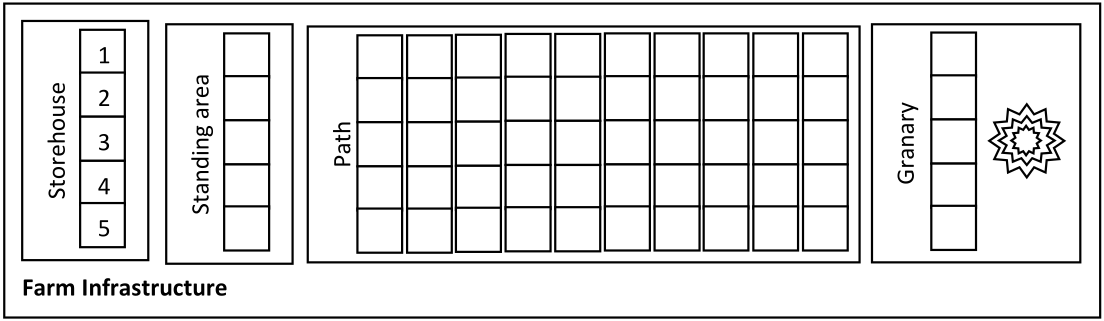
\includegraphics[width=\linewidth]{img/Design_FI.png}
%   \end{minipage}%
%   \caption{Visual representation of the farm, taken from \cite{assign}.}
%   \label{Design_FI}
% \end{figure} 

%\texttt{java -cp <userdir>/build/classes fi.FarmInfrastructure}

\newpage
\section{Scientific Computation and Custom Systems} %%%%%%%%%%%%%%%%%%%%%%%%%%%%%%%%%%%%%%%%%%%%%%%%%%%%%%%%%%%%%%%%%%%%%%%%%%%%%%%%%%%%%%%%%%%%%%%%%%%%%%%%%%%%%%%%%%%%%


\subsection{The Scenario} %%%%%%%%%%%%%%%%%%%%%%%%%%%%%%%%%%%%%%



\subsection{The Messages} \label{messages} %%%%%%%%%%%%%%%%%

\section{System Architecture} %%%%%%%%%%%%%%%%%%%%%%%%%%%%%%%%%%%%%%%%%%%%%%%%%%%%%%%%%%%%%%%%%%%%%%%%%%%%%%%%%%%%%%%%%%%%%%%%%%%%%%%%%%%%%%%%%%%%%%%%%%%%%%%%%%


\subsection{Entities} \label{entitites} %%%%%%%%%%%%%%%%%%%%


\subsection{Components} \label{components} %%%%%%%%%%%%%%%%%


\subsection{User Interface} %%%%%%%%%%%%%%%%%%%%%%%%%%%%%%%%


\section{Architecture Constraints} \label{infrastructure} %%%%%%%%%%%%%%%%%%%%%%%%%%%%%%%%%%%%%%%%%%%%%%%%%%%%%%%%%%%%%%%%%%%%%%%%%%%%%%%%%%%%%%%%%%%%%%%%%%%%%%%%%%


\subsection{Quality Attributes Assurance} %%%%%%%%

\subsection{User Cases Compliance} %%%%%%%%

\newpage
\section{Additional Remarks} %%%%%%%%%%%%%%%%%%%%%%%%%%%%%%%%%%%%%%%%%%%%%%%%%%%%%%%%%%%%%%%%%%%%%%%%%%%%%%%%%%%%%%%%%%%%%%%%%%%%%%%%%%%%%%%%%%%%%%%%%%%%%%%%%%%

\subsection{Documentation} %%%%%%%%%%%%%%%%%%%%%%%%%%%%%%%%%

Our attitude towards the developed code was to ensure it could be applied to other similar scenarios and reused in systems intended to be deployed in real scenarios.
With this in mind, we took great care with regards to code readability.
By maintaining a code style equal throughout the project and defining intuitive and self-explaining variable and method names, we made the code easy to understand
by someone already contextualized with Kafka.

Nevertheless, we wanted to make sure this was also true to someone looking at our project for the first time, so we resorted to the well-known Javadoc
\cite{javadoc} tool to manage all code documentation.
Comments were also added in key points throughout the code, including the scripts.

\subsection{Assignment Contributions} %%%%%%%%%%%%%%%%%%%%%%

As the entire development phase took place in a time where on-site cooperation was not possible, we resorted to online communication platforms to debate decisions
and discuss difficulties.
Team scheduling allowed us to work on the project simultaneously, so no member suffered from unbalanced workloads.
The dimension of the project did not appeal to the usage of repository pull requests and other synchronization tools.
However, each small solution was verified and agreed by both team members.

Having said this, it is difficult to isolate what each member actually implemented, as the influence of both is present in all components.
Nevertheless, one might say that each had stronger responsibilities on a set of project aspects:
Filipe took care of the execution of the individual Java processes and of the Shell scripts, while João developed the Kafka-related classes such as Consumer,
Producer and EntityAction; Filipe developed the Python script for generation of \texttt{CAR.TXT}, while João developed the Shell scripts for Kafka initialization
and deletion; each implemented 2 entities and each wrote a portion of this report; Filipe made sure everything was coherent throughout the report and the code
documentation, while João solved the most critical issues regarding the configuration of the topics.
In terms of work percentage, we believe it was about 50\% for each student.

\newpage
\section*{Conclusions} %%%%%%%%%%%%%%%%%%%%%%%%%%%%%%%%%%%%%%%%%%%%%%%%%%%%%%%%%%%%%%%%%%%%%%%%%%%%%%%%%%%%%%%%%%%%%%%%%%%%%%%%%%%%%%%%%%%%%%%%%%%%%%%%%%%%%%%%%

\begin{thebibliography}{9} %%%%%%%%%%%%%%%%%%%%%%%%%%%%%%%%%%%%%%%%%%%%%%%%%%%%%%%%%%%%%%%%%%%%%%%%%%%%%%%%%%%%%%%%%%%%%%%%%%%%%%%%%%%%%%%%%%%%%%%%%%%%%%%%%%%%%
  \bibliographystyle{Science}

  % \bibitem{uml}
  %   Object Management Group,
  %   \textit{What is UML},
  %   \url{https://www.uml.org/what-is-uml.htm},
  %   accessed in March 2020.



\end{thebibliography}

\clearpage

\end{document}




















